\documentclass[german]{book}
%\usepackage{url}
\PassOptionsToPackage{hyphens}{url}\usepackage[breaklinks=true]{hyperref}
\usepackage{dsfont}
\usepackage{listings}
\usepackage{german}
\usepackage[utf8]{inputenc}
\usepackage[final]{graphicx}

% beide packages eingefügt um Referenzen für Abbildungen nutzen zu können
\usepackage{hyperref}
\usepackage[ngerman,nameinlink]{cleveref}

\begin{document}

\section{Dokumentengeschichte}
\begin{table}[h]
 \begin{tabular}{|l|l|p{4cm}|}
 \hline
 Zeitraum & PL/Autor(en) & Änderungen \\
 \hline
 Sommersemester 1980 & IHR NAME & 
text \newline 
 
  \\
 \hline
 Wintersemester 2017/18 & Jan Schuster & 
Erstellung eines Konzeptes zur Nutzerverwaltung
\newline 

 
  \\
 \hline
 \end{tabular}
 \caption{Dokumentengeschichte}
 \end{table}

\section{Aufgabe der Komponente}
Diese Komponente soll eine Grundlage für die spätere Entwicklung eines Webservers liefern. Darin enthalten, soll sein,  ein Prototypisches Verhalten für die Benutzerverwaltung und die Kommunikation über Rest Schnittstellen. Ein Nutzerprogramm soll dabei die Möglichkeit erhalten, sich auf den Server zu authentifizieren und entsprechend seiner Rechte, Daten lesen oder schreiben können. Die Kommunikation soll über REST stattfinden. Außerdem soll sie über Apache Tomcat Lauffähig sein. 
\newline
\newline
Das Grundlegende Ziel ist es, diese Authentifizierung mit so wenig externen Komponenten wie möglich zu bauen. 

\newpage

\section{Architektur}
\subsection{Überlick} 
Die grundlegenden Nutzerdaten werden in einer UserBean vorgehalten. Das Singleton UserBase kümmert sich um die Verwaltung der Nutzer. Beim Initialisieren werden alle Nutzer in einer Collection gepackt und es wird ein Timer in die jeweilige Bean aus der UserBase mit rein gegeben.  Wird ein Remembertoken in der UserBean gesetzt, wird ein Thread mit einen Timertask erzeugt. Beim erneuten setzen des Timers, wird der Thread auf den Ursprung zurück gesetzt. Jegliche Anfragen zu einen Benutzer findet ausschließlich über die Instanz des Singletons UserBase statt. Das bearbeiten oder verändern von Benutzern verantworten die Schnittstellen selbst. 
\newline
\newline
Es gibt zwei Klassen die REST Schnittstellen zur Verfügung stellen. Die erste ist die Klasse AuthResource und die zweite die UserResource. Folgende Use-Cases sind durch die beiden Klassen abgedeckt:
\newline
\newline
AuthResource:
\newline
- Methode zum Testen der regulären Rest Funktion
\newline
- Methode zum Authentifizieren von Nutzerdaten ->eventuelle Rückgabe eines Tokens zur weiteren Verwendung
\newline
\newline
UserResource:
\newline
- Methode zur Ausgabe von Nutzerdaten anhand eines herein gegebenen Nutzers
\newline
- Methode zum Setzen eines Passwortes für einen Nutzer anhand eines Tokens und eines Passwortes
\newline
- Methode zum anzeigen der Rechte eines Tokens anhand des herein gegebenen Tokens
\newline
\newline
\newpage
Beispiel eines Authorisierungsprozesses: 
\newline
\newline
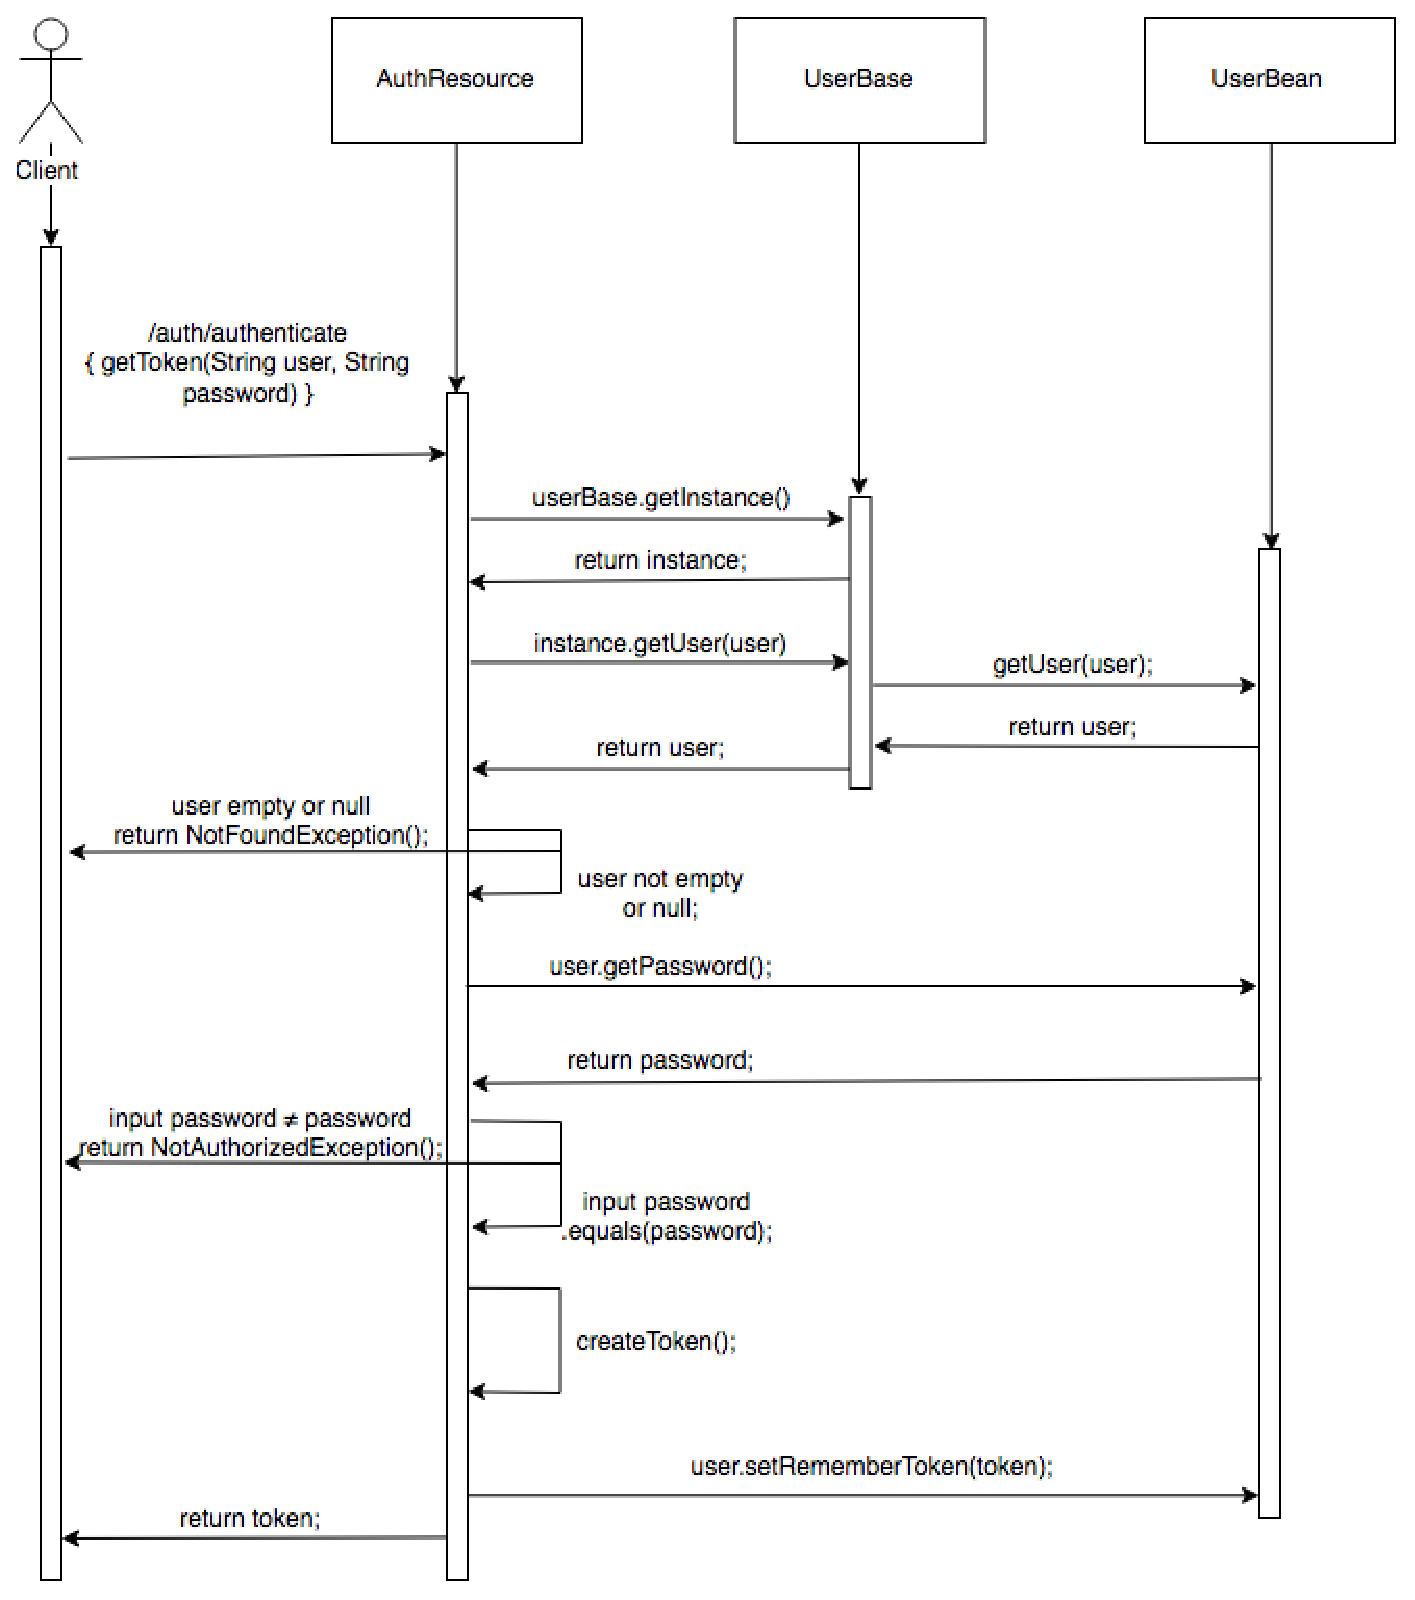
\includegraphics[scale=0.6]{auth-process.eps}


\newpage
\subsection{Schnittstellendefinitionen}

\subsubsection{Authentifizierung: AuthResource}
Die erste ist eine Default Test Methode zum testen der allgemeinen Funktionsfähigkeit und gibt einen String mit "Default REST Method" zurück. 
\newline
Methodenname: restTest()
\newline
Schnittstelle: /auth/test
\newline
Medien Typ: Text\_Html, Text\_Plain
\newline
\newline
Die zweite Methode ist für die Authentifizierung gedacht. Die Schnittstelle selbst bekommt einen Nutzer und ein Passwort als Eingabe herein. Als erstes wird überprüft ob auch ein Nutzer in die Methode gegeben wurde. Ist dies der Fall, wird sich eine Instanz der UserBase geholt. Danach wird überprüft ob ein Password herein gegeben wurde und ob dieses mit dem zur Verfügung gestellten Benutzer übereinstimmt. 
\newline
\newline
Ist dies der Fall, wird ein String aus dem Nutzer, dem Password und einer Random UUID erstellt.  Aus diesem String wird mit Hilfe des Base 64 Encoder ein 
ein Token erzeugt. Daraufhin wird eine Methode im Nutzer selbst getriggert, die den Token als RememberToken speichert und ein Timer aktiviert, der die gültige Zeitdauer des Tokens bestimmt. Zum Schluss wird der Token selbst als String zurückgegeben.
\newline
Methodenname: getToken(String user, String password)
\newline
Schnittstelle: /auth/authenticate
\newline
Medien Typ: Text\_Html, Text\_Plain

\subsubsection{Nutzer: UserResource}
Die erste Methode ist als Rückgabe der angefragten Nutzerdaten als JSON gedacht. Der Methode wird nur ein Nutzer übergeben. Daraufhin wird überprüft, ob der Nutzer im System vorhanden ist. Ist dies der Fall, werden die Daten mithilfe der MediaType in eine JSON umgewandelt. 
\newline
Methodenname: getUser(String user)
\newline
Schnittstelle: /user/getUser
\newline
Medien Typ: Application\_JSON
\newline
\newline
Die Zweite Methode ist für das Setzen eines Passwortes im System zugehörig zu einem bestimmten Nutzer gedacht. Dazu werden in die Methode, der Identifizierungstoken und das neue Password herein gegeben. Als erstes wird überprüft ob der Token im System vorhanden ist. Ist dies der Fall, wird sich die Instanz des Nutzers zugehörig zum Token geholt. Danach wird das Passwort des Nutzers neu gesetzt sowie auch die Funktion setRememberToken mit dem Token aufgerufen. Das Triggert erneut den Timer und setzt ihn auf die Ursprungszeit zurück. Als Rückgabe wird der veränderte Nutzer als JSON ausgegeben.
\newline
Methodenname: setPassword(String token, String password)
\newline
Schnittstelle: /user/setPassword
\newline
Medien Typ: Application\_JSON
\newline
\newline
Die dritte Methode ist dafür da, sich den Nutzer und dessen Rechte anhand des bereitgestellten Tokens anzusehen. Als erstes wird der Token überprüft, ob er im System vorhanden ist. Ist dies der Fall, werden die Nutzerdaten, inklusive Rechte, als JSON zurückgegeben. 
\newline
Methodenname: myRights(String token)
\newline
Schnittstelle: /user/myRights
\newline
Medien Typ: Application\_JSON
\newline
\newline

\subsection{genutzte Komponenten}

\subsubsection{Glassfish Jersey}
Dient als Webserver Applikation im Tomcat. Kann durch beliebigen anderen, im Tomcat Container laufenden Webserver ausgetauscht werden. (Bsp.: Jetty, Spring Boot) Daher wird hier nicht weiter auf die Versionierung eingegangen. Der Applikationsserver muss aber das Package javax.ws.rs zur Verfügung stellen.

\subsubsection{Base64Encoder}
Wird zur Erzeugung der Token genutzt. Ist im Package java.util.Base64 enthalten.

\subsubsection{Java UUID}
Wird für die Generierung der Random UUID genutzt. Ist im Package java.util.UUID enthalten.

\section{Nutzung}
\subsection{Code}



\subsection{Deployment / Runtime}
Aus dem Quellcode lässt sich mithilfe von dem Befehl "mvn package" eine WAR Datei erstellen. Dies ist möglich da Maven als Paket Manager eingesetzt wurde. Anschließend lässt sich die WAR auf jeden laufenden Tomcat Server einbinden. 
\newline
\newline
Beschreibung wie die Komponenten aus dem Quellcode erzeugt werden kann,
wie sie installiert wird und wie man sie startet.

\section{Qualitätssicherung}
Innerhalb der Abfragen wird überprüft, ob Eingaben vorhanden sind und ob diese mit den schon vorhandenen Daten übereinstimmen. Ist dies nicht der Fall, werden entsprechende Fehlermeldungen geworfen. Für die Spätere Entwicklung des Authentifizierungsservers werden aber Service und Unit Tests empfohlen. 

\subsection{Test}
Finden ausschließlich per Hand mit dem Browser statt. 

\section{Vorschläge / Ausblick}
Hier wurde Prototypisch aufgezeigt wie eine Authentifizierung stattfinden kann. Sobald die Implementierung mit der Datenbank und der Clients Stattfindet, wird empfohlen ein entsprechendes BCrypt Format zu integrieren. (z.B. JBCrypt). Dieses dient zur Verhashung des Passworts und verhindert das ein Passwort direkt aus der Datenbank ausgelesen werden kann oder in Klartext übertragen wird. 
\newline
\newline
\end{document}